\chapter{Biodiversità e unità chimica}

Le molecole biologiche sono molto complesse, ma sono costruite da un
numero limitato di elementi. Le biomolecole diverse sono caratterizzati
da determinati gruppi funzionali e da diversi legami. Durante
l'evoluzione biologica i composti semplici si sono uniti per formare
molecole più complesse e polimeri. Una caratteristica importante è la
capacità di autoreplicarsi.

\marginpar{
    \begin{tabular}{cc}
        Elemento & Peso secco in \% \\
        \ce{C} & 61.7\\
        \ce{N} & 11.0\\
        \ce{O} & 9.3\\
        \ce{Ca} & 5\\
        \ce{P} & 3.3\\
        \ce{K} & 1.3\\
        \ce{S} & 1\\
        \ce{Cl} & 0.7\\
        \ce{Na} & 0.7\\
        \ce{Mg} & 0.3\\
    \end{tabular}
    \captionof{table}{Elementi più presenti nelle molecole biologiche}
}

Esiste una gerarchia costruttiva e tutte le forme di vita sono
costituite da stessi elementi, tipi di molecole, che si organizzano in
polimeri aggregati e strutture supramolecolari, ossia in strutture via
via sempre più complesse e dunque caratterizzante

\begin{figure}[H]
    \centering
    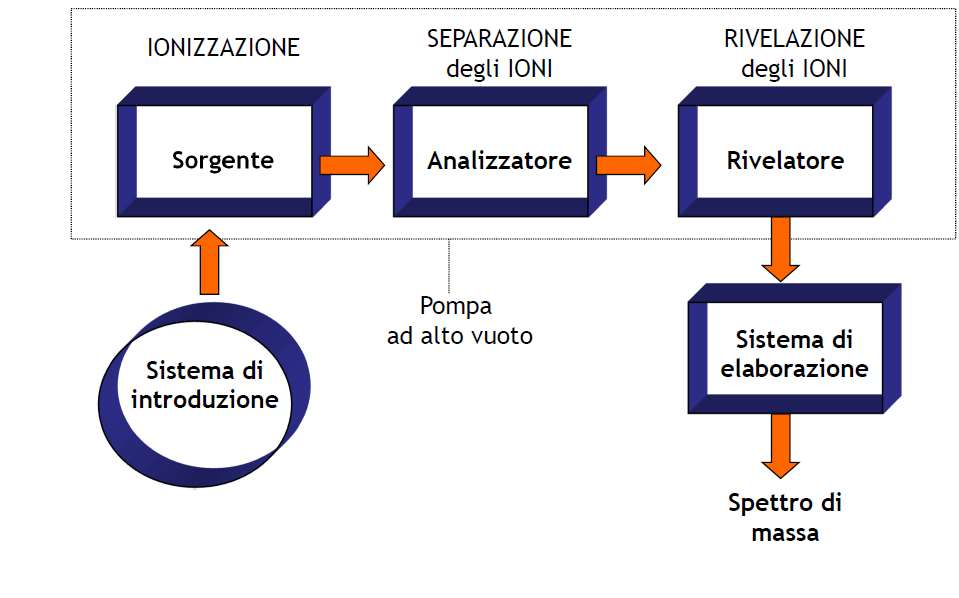
\includegraphics[width=0.8\textwidth]{2_001}
    \caption{Gerarchia costtruttiva}
\end{figure}

\clearpage

\section{Cellula}

\fullpicture*{2_002}{Cellula procariote}

La cellula è l'unità minima per definire uno stato vivente. Le cellule
più semplici sono quelle dei procarioti, che sono unicellulari e la loro
cellula non presenta un nucleo, ma possiede solo il citoplasma, il DNA e
alcuni organelli di base. Queste cellule sono molto piccole, infatti si
aggirano intorno a 10--100 \mu m. Queste cellule sono proprie di diversi
tipi di batteri, come gli eubatteri e gli archeobatteri.

I ribosomi sono delle proteine che catalizzano la sintesi di altre
proteine

Gli eucarioti invece hanno un nucleo e possono essere sia unicellulari
che pluricellulari. A differenza delle cellule procariotiche, le cellule
eucariotiche hanno diversi compartimenti specializzati (ovvero gli
organelli) per delle reazioni specifiche, mentre nei procarioti le
reazioni avvengono nel citoplasma.

Il nucleo contiene il DNA separato dal resto della molecola da una
membrana nucleare; è circondato da un reticolo, detto ``reticolo
endoplasmatico''. All'interno della cellula sono presenti:
\begin{itemize}
    \item \emph{Mitocondri},
    che fungono da centrali energetiche cellulari,
    \item \emph{Ribosomi}, che sono
    all'interno del reticolo endoplasmatico, 
    \item \emph{Lisosomi}, che svolgono la
    funzione di degradare le proteine che non sono più utili e che quindi
    sono pericolose per la cellula 
    \item \emph{Apparato del Golgi}, che serve per
    sintetizzare altre proteine
    \item \emph{Membrana plasmatica}, che separa la cellula
    dall'ambiente extracellulare
\end{itemize}

Le cellule vegetali hanno i cloroplasti, ovvero degli organelli deputati
alla fotosintesi, inoltre hanno un vacuolo centrale molto grande, che
contiene acqua. Quando il vacuolo è pieno fornisce il turgore che
contraddistingue le cellule animali da quelle vegetali. Inoltre, le
cellule vegetali possiedono una parete cellulare, che è più resistente
della membrana plasmatica

\fullpicture*{2_003}{Cellula eucariote animale}

\fullpicture*{2_004}{Cellula eucariote vegetale}

Gli elementi chimici utilizzati sono principalmente il carbonio, in
quanto questo consente dei legami molto stabili; inoltre è un elemento
molto versatile.

\fullpicture*{2_005}{Gerarichia costruttiva della cellula}

\section{Acqua}

\marginpicture*{2_006}{Acqua}

Il solvente della vita è l'acqua, in quanto il citoplasma della cellula
è l'acqua. Questo si vede nel fatto che gli organismi sono formati da
una gran parte di acqua (nell uomo circa il 70 \%). L'acqua quindi è
essenziale e quindi è necessario studiare le caratteristiche dell'acqua
per tre motivi: 
\begin{itemize}
    \item Quasi tutte le molecole assumono una forma (struttura)
    e quindi una funzione, in risposta alle proprietà chimiche e fisiche
    dell'acqua 
    \item L'acqua è il mezzo in cui avviene la maggior parte delle
    reazioni e i reagenti e i prodotti sono trasportati dall'acqua
    all'interno delle cellule
    \item L'acqua partecipa attivamente a molti tipi
    di reazione
\end{itemize}

Inoltre, spesso a reagire si trovano gli ioni \ce{H+} e
\ce{OH-}, quindi si vede che la reattività di molti composti è funzione
del pH.

\subsection{Proprietà dell'acqua}

L'acqua è una molecola polare con un momento di dipolo di 1.83. L'acqua
è quindi in grado di formare legami ad idrogeno.

L'acqua è inglobata nella macromolecole proprio grazie a legami ad
idrogeno. Allo stato solido, le molecole d'acqua sono mantenute in una
disposizione cristallina creata dai legami ad idrogeno. In questa
disposizione, ogni molecola forma quattro legami ad idrogeno con altre
molecole di acqua.

\halfpicture*{2_007}{Legame ad idrogeno nell'acqua}

Nello stato liquido, invece, i legami ad idrogeno si formano e si
rompono velocemente, quindi il reticolo che si forma è irregolare.
Questo comporta anche che la densità del ghiaccio sia minore rispetto a
quella dell'acqua liquida; se così non fosse non sarebbe possibile la
vita in acqua.

L'acqua scioglie molecole polari, composti ionici e molecolari che
possono formare legami ad idrogeno. L'acqua allenta la forza coulombiana
che tiene legati i solidi ionici.

L'acqua è in grado di passare attraverso le membrane semipermeabili,
come ad esempio la membrana plasmatica. Questo spostamento è dovuto alla
differenza dei potenziali chimici delle due soluzioni. Questo fenomeno
prende nome di ``pressione osmotica''.

\fullpicture*{2_008}{L'acqia si mouve per osmosi}

Per evitare che la cellula scoppi, le cellule animali sono immerse in
soluzioni con un potenziale chimico simile, mentre le cellule animali
sono più resistenti

L'acqua funge anche da solvente negli equilibri acido-base. Il valore
della \(pK_a\) dipende, oltre che dal tipo di acido, anche
dall'ambiente, dall'attrazione delle cariche e dall'idratazione degli
ioni.

Quando \(pH \approx pK_a\), si è in una zona del \(pH\) detta tampone.
Ad esempio, per l'acido fosforico, ovvero \ce{H3PO4}, si hanno tre zone
tampone, corrispondenti alle tre dissociazioni acide
\[
    pK_1=2.14 \quad pK_2=6.36 \quad pK_3=12.4
\]

La seconda \(pK_a\) dell'acido fosforico ha un valore molto simile al pH
fisiologico; la coppia di sali \ce{H2PO4-} e \ce{HPO4^{2-}} è utilizzata
per i tamponi a \(pH\) vicini a \(pH=7\). Degno di nota è anche l'acido
carbonico, per cui esiste la reazione di equilibrio:
\[
\ce{CO2 + H2O <=> H2CO3 <=> H+ + HCO3-} \quad pK_a=6.35 \:
\text{complessivo}
\]
Questo equilibrio è l'equilibrio più importante
che avviene nel sangue.

Gli ioni fosfato e carbonato sono presenti in quasi tutti i fluidi
biologici. Sono importanti agenti tamponanti, in quanto i valori delle
loro \(pK_a\) sono compresi nell'intervallo del \(pH\) fisiologici.
Questo si vede anche dall'equazione di Henderson
\[
pH = pK_a + \log \frac{[A^-]}{[HA]}
\]

\fullpicture*{2_009}{Titolazione dell'acido forforico}

Il pH fisiologico, come già detto prima, è vicino a 7, tranne in alcuni
casi. Un caso è quello del pH dei succhi gastrici, che è molto basso;
questo avviene perché nella digestione sono richiesti dei valori di pH
molto acidi per la denaturazione delle proteine e per altre reazioni che
avvengono durante la digestione.

Il pH dell'oceano è di circa 8, l'anidride carbonica sta aumentando.
Questo comporta che il pH dell'oceano stia diminuendo, in quando
l'anidride carbonica viene solvatata in acqua e, tramite equilibrio
acido-base, forma lo ione bicarbonato/carbonato, con rilascio di
\ce{H+}. Questo fenomeno prende il nome di ``acidificazione degli
oceani''.

Le alterazioni, anche minime, delle condizioni di equilibrio possono
sconvolgere gli equilibri biologici con conseguenze imprevedibili, come
nel caso di alcune forme di vita marine che, per via dell'acidificazione
degli oceani, non riescono a produrre il loro esoscheletro (guscio).

\marginpicture*{2_010}{Range di pH}

\section{Molecole anfipatiche}

Queste molecole hanno una parte idrofobica e una idrofilica

\begin{figure}[H]
    \centering
    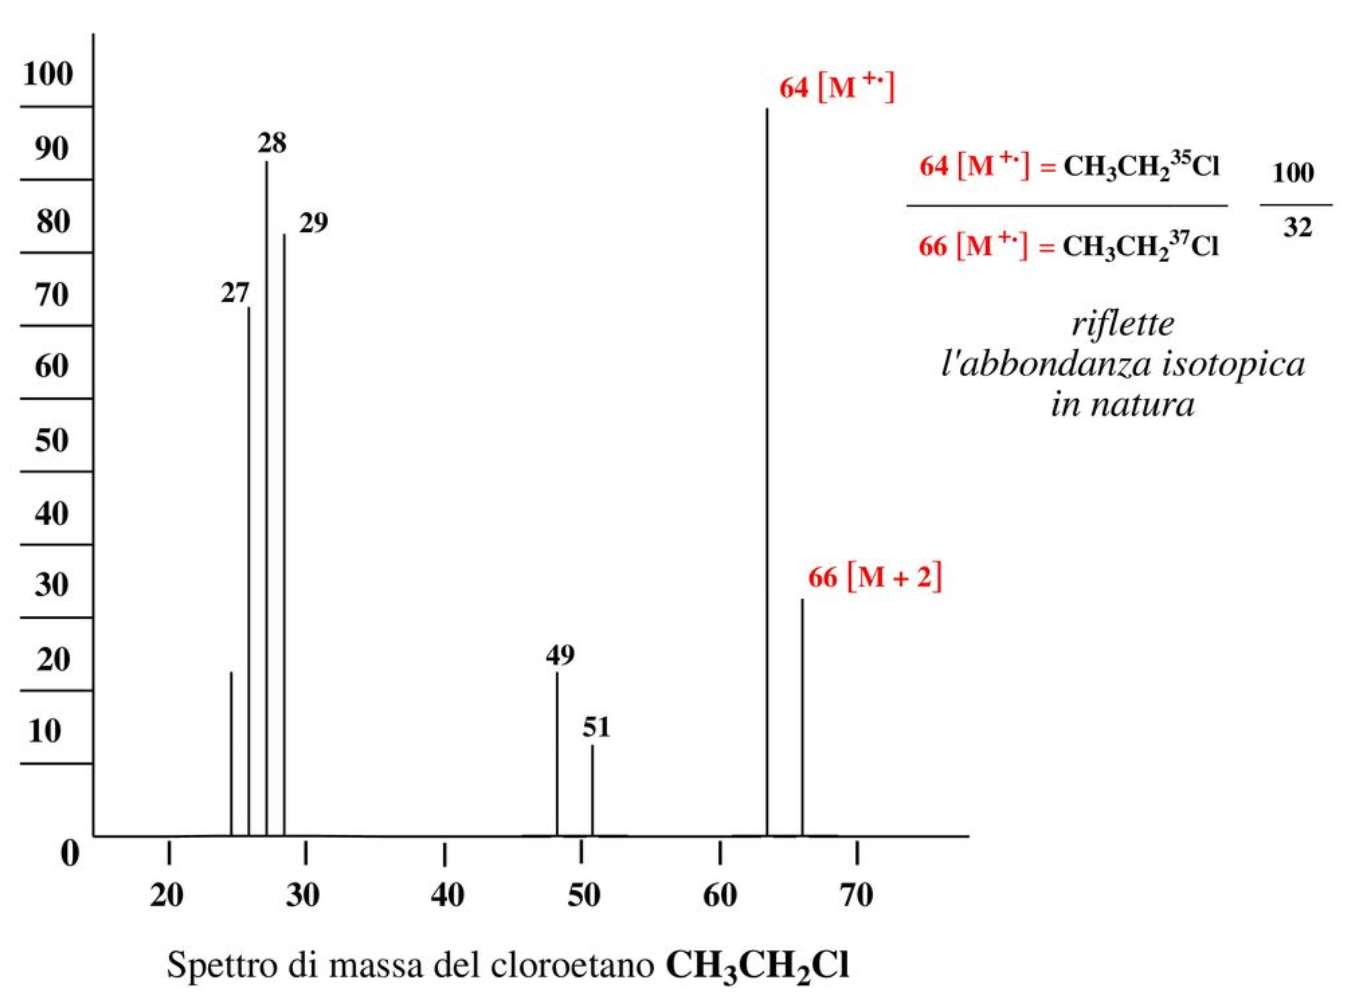
\includegraphics[width=0.5\textwidth]{2_011}
\end{figure}

Queste molecole si dispongono in una distribuzione ben definita dettata
da motivi entropici. I casi possibili sono due:
\begin{itemize}
    \item Micelle 
    \item A doppio strato
\end{itemize} 

Si crea in questo modo una membrana semipermeabile utile per separare la
cellula dall'esterno.

\fullpicture*{2_012}{Possibili disposizioni delle molecole anfipatiche, ovvero a micelle e a doppio strato.}

\subsection{Considerazioni termodinamiche}

Gli organismi sono sistemi aperti di non equilibrio. In una cellula, tutte le reazioni sono spontanee \(\Delta G < 0\). Essendo un ambiente non all'equilibrio, gli organismi per stare in uno
stato stazionario scambiano costantemente materia ed energia con
l'ambiente circostante.
Le condizioni standard in biologia sono: 25°C, 1 atm e pH=7

Ricordando la legge termodinamica
\[
\Delta G = \Delta H - T\Delta S
\]
Si vede che molte reazioni siano sfavorite termodinamicamente, come
ad esempio la produzione di ATP, che però possono essere forzate con un
cambiamento entropico. Per catalizzare le reazioni sono presenti degli
enzimi, che aumentano la velocità della reazione.{}